%%%% ijcai19.tex

\typeout{IJCAI-19 Instructions for Authors}

% These are the instructions for authors for IJCAI-19.

\documentclass{article}
\pdfpagewidth=8.5in
\pdfpageheight=11in
% The file ijcai19.sty is NOT the same than previous years'
\usepackage{ijcai19}

% Use the postscript times font!
\usepackage{times}
\usepackage{soul}
\usepackage{url}
\usepackage[hidelinks]{hyperref}
\usepackage[utf8]{inputenc}
\usepackage[small]{caption}
\usepackage{graphicx}
\usepackage{amsmath}
\usepackage{booktabs}
\usepackage{algorithm}
\usepackage{algorithmic}
\usepackage{xspace}
\urlstyle{same}

%%%%%%%%%%%%%%%%%% Added for this paper
\usepackage{enumitem}
\usepackage{amsthm}
\usepackage{amssymb}
\usepackage{listings}% http://ctan.org/pkg/listings
\lstset{
  basicstyle=\ttfamily,
  mathescape
}
\usepackage{ wasysym }
\newcommand{\tup}[1]{{\langle #1 \rangle}}
\newcommand{\pre}{\mathsf{pre}}     % precondition
\newcommand{\del}{\mathsf{del}}     % effect
\newcommand{\add}{\mathsf{add}}     % effect
\newcommand{\eff}{\mathsf{eff}}     % effect
\newcommand{\cond}{\mathsf{cond}}   % conditional effect
\newcommand{\true}{\mathsf{true}}   % true
\newcommand{\false}{\mathsf{false}} % false
\newcommand{\PE}{\mathrm{PE}}     % precondition
\newcommand{\strips}{\textsc{Strips}}

\newcommand{\ARMS}{{\small {\sffamily ARMS}}\xspace}
\newcommand{\CAMA}{{\small {\sffamily CAMA}}\xspace}
\newcommand{\SLAF}{{\small {\sffamily SLAF}}\xspace}
\newcommand{\LAMP}{{\small {\sffamily LAMP}}\xspace}
\newcommand{\NOISTA}{{\small {\sffamily NOISTA}}\xspace}
\newcommand{\LOCM}{{\small {\sffamily LOCM}}\xspace}
\newcommand{\LOCMtwo}{{\small {\sffamily LOCM2}}\xspace}
\newcommand{\LOP}{{\small {\sffamily LOP}}\xspace}
\newcommand{\AMAN}{{\small {\sffamily AMAN}}\xspace}
\newcommand{\LOUGA}{{\small {\sffamily LOUGA}}\xspace}


\newtheorem{mytheorem}{Theorem}
\newtheorem{mylemma}[mytheorem]{Lemma}
\newtheorem{mydefinition}[mytheorem]{Definition}

%%%%%%%%%%%%%





% the following package is optional:
%\usepackage{latexsym}

% Following comment is from ijcai97-submit.tex:
% The preparation of these files was supported by Schlumberger Palo Alto
% Research, AT\&T Bell Laboratories, and Morgan Kaufmann Publishers.
% Shirley Jowell, of Morgan Kaufmann Publishers, and Peter F.
% Patel-Schneider, of AT\&T Bell Laboratories collaborated on their
% preparation.

% These instructions can be modified and used in other conferences as long
% as credit to the authors and supporting agencies is retained, this notice
% is not changed, and further modification or reuse is not restricted.
% Neither Shirley Jowell nor Peter F. Patel-Schneider can be listed as
% contacts for providing assistance without their prior permission.

% To use for other conferences, change references to files and the
% conference appropriate and use other authors, contacts, publishers, and
% organizations.
% Also change the deadline and address for returning papers and the length and
% page charge instructions.
% Put where the files are available in the appropriate places.

\title{One-shot learning: From domain knowledge to action models}

% Single author syntax
%\author{
%    Sarit Kraus
%    \affiliations
%    Department of Computer Science, Bar-Ilan University, Israel \emails
%    pcchair@ijcai19.org
%}

% Multiple author syntax (remove the single-author syntax above and the \iffalse ... \fi here)
% Check the ijcai19-multiauthor.tex file for detailed instructions
\author{
Diego Aineto$^1$\and
Sergio Jim\'enez$^1$\and
Eva Onaindia$^1$
\affiliations
$^1${\small Departamento de Sistemas Inform\'aticos y Computaci\'on. Universitat Polit\`ecnica de Val\`encia. Valencia, Spain}
\emails
{\scriptsize \{dieaigar,serjice,onaindia\}@dsic.upv.es}}


\begin{document}
\maketitle


\begin{abstract}
Most approaches to learning action planning models heavily rely on a significantly large volume of training samples or plan observations. In this paper, we adopt a different approach based on deductive learning from domain-specific knowledge, specifically from logic formulae that specify constraints about the possible states of a given domain. The minimal input observability required by our approach is a single example composed of a full initial state and a partial goal state. We will show that exploiting specific domain knowledge enable to constrain the space of possible action models as well as to complete partial observations, both of which turn out helpful to learn good-quality action models.
 \end{abstract}



\section{Introduction}
\label{sec:introduction}

The learning of action models in planning has been typically addressed with inductive learning data-intensive approaches. From the pioneer learning system \ARMS~\cite{yang2007learning} to more recent ones \cite{MouraoZPS12,zhuo2013action,kuvcera2018louga}, all of them require thousands of plan observations or training samples, i.e., sequences of actions as evidence of the execution of an observed agent, to obtain and validate an action model. These approaches return the statistically significant model that best explains the plan observations by minimizing some error metric. A model explains an observation if a plan containing the observed actions can be generated with the model and the states induced by this plan also include the possibly partially observed states. The limitation of posing model validation as an optimization task over a testing set of observations is that it neither guarantees completeness (the model may not explain all the observations) nor correctness (the states induced by the execution of the plan generated with the model may contain contradictory information).

Differently, other approaches rely on symbolic-via learning. The Simultaneous Learning and Filtering (\SLAF) approach~\cite{AmirC08} exploits logical inference and builds a complete explanation through a CNF formula that represents the initial belief state, and a plan observation. The formula is updated with every action and state of the observation, thus representing all possible transition relations consistent with it. \SLAF extracts all satisfying models of the learned formula with a SAT solver although the algorithm cannot effectively learn the preconditions of actions. A more recent approach addresses the learning of action models from plan observations as a planning task which searches the space of all possible action models~\cite{aineto2018learning}. A plan here is conceived as a series of steps that determine the preconditions and effects of the action models plus other steps that validate the formed actions in the observations. The advantage of this approach is that it only requires input samples of about a total of 50 actions.

This paper studies the impact of using mixed input data, i.e, automatically-collected plan observations and human-encoded domain-specific knowledge, in the learning of action models. Particularly, we aim to stress the extreme case of having a single observation sample and answer the question to whether the lack of training samples can be overcome with the supply of domain knowledge. The question is motivated by (a) the assumption that obtaining enough training observations is often difficult and costly, if not impossible in some domains~\cite{Zhuo15}; (b) the fact that although the physics of the real-world domain being modeled are unknown, the user may know certain pieces of knowledge about the domain; and (c) the desire for correct action models that are usable beyond their applicability to a set of testing observations. To this end, we opted for checking our hypothesis in the framework proposed in~\cite{aineto2018learning} since this planning-based satisfiability approach allows us to configure additional constraints in the compilation scheme, it is able to work under a minimal set of observations and uses an off-the-shelf planner\footnote{We thank authors for providing us with the source files of their learning system.}. Ultimately, we aim to compare the informational power of domain observations (information quantity) with the representational power of domain-specific knowledge (information quality). Complementarily, we restrict our attention to solely observations over fluents as in many applications the actual actions of an agent may not be observable~\cite{SohrabiRU16}.

Next section summarizes basic planning concepts and outlines the baseline learning approach~\cite{aineto2018learning}. Then we formalize our one-shot learning task with domain knowledge and subsequently we explain the task-solving process. Section 5 presents the experimental evaluation and last section concludes.



\section{Background}
\label{sec:background}

We denote as $F$ (fluents) the set of  propositional state variables. A partial assignment of values to fluents is represented by $L$ (literals). We adopt the \emph{open world assumption} (what is not known to be true in a state is unknown) to implicitly represent the unobserved literals of a state. Hence, a state $s$ includes positive literals ($f$) and negative literals ($\neg f$) and it is defined as a full assignment of values to fluents; $|s|=|F|$. We use $\mathcal{L}(F)$ to denote the set of all literal sets on $F$; i.e.~all partial assignments of values to fluents.

A {\em planning action} $a$ has a precondition list $\pre(a)\in\mathcal{L}(F)$ and a effect list $\eff(a)\in\mathcal{L}(F)$. The semantics of an action $a$ is specified with two functions: $\rho(s,a)$ denotes whether $a$ is {\em applicable} in a state $s$ and $\theta(s,a)$ denotes the {\em successor state} that results of applying $a$ in a state $s$. Then, $\rho(s,a)$ holds iff $\pre(a)\subseteq s$, i.e.~if its precondition holds in $s$. The result of executing an applicable action $a$ in a state $s$ is a new state $\theta(s,a)=\{s\setminus \neg\eff(a)\cup\eff(a)\}$, where $\neg\eff(a)$ is the complement of $\eff(a)$, and it is subtracted from $s$ so as to ensure that $\theta(s,a)$ remains a well-defined state.

%The subset of action effects that assign a positive value to a state fluent is called {\em positive effects} and denoted by $\eff^+(a)\in \eff(a)$ while $\eff^-(a)\in \eff(a)$ denotes the {\em negative effects} of an action $a\in A$.

A {\em planning problem} is a tuple $P=\tup{F,A,I,G}$, where $I$ is the initial state and $G\in\mathcal{L}(F)$ is the set of goal conditions over the state variables. A {\em plan} $\pi$ is an action sequence $\pi=\tup{a_1, \ldots, a_n}$, with $|\pi|=n$ denoting its {\em plan length}. The execution of $\pi$ in $I$ induces a {\em trajectory} $\tup{s_0, a_1, s_1, \ldots, a_n, s_n}$ such that $s_0=I$ and, for each {\small $1\leq i\leq n$}, it holds $\rho(s_{i-1},a_i)$ and $s_i=\theta(s_{i-1},a_i)$. A plan $\pi$ solves $P$ iff the induced trajectory reaches a final state $s_n$ such that $G \subseteq s_n$.

The baseline learning approach (hereafter \textbf{BLA} for short) our proposal draws upon uses {\em actions with conditional effects}~\cite{aineto2018learning}. The conditional effects of an action $a_c$ is composed of two sets of literals: $C\in\mathcal{L}(F)$, the {\em condition}, and $E\in\mathcal{L}(F)$, the {\em effect}. The {\em triggered effects} resulting from the action application (conditional effects whose conditions hold in $s$) is defined as $\eff_c(s,a)=\bigcup_{C\rhd E\in\cond(a_c),C\subseteq s} E$.

\subsection{Learning action models with classical planning}
\label{FAMA}

The {\em classical planning compilation} for the learning of \strips\ action models~\cite{aineto2018learning} receives as input an {\em empty} model (which contains just the {\em name} and {\em parameters} of each action schema), and a set of observations of plan executions. The compilation completes the {\em empty} model specifying the preconditions and effects of each action schema such that the validation of the completed model over the input observations is successful; i.e., there exists a plan computable with the completed model s.t. $\rho(s_{i-1}^o,a_i)$ and $s_i^o=\theta(s_{i-1}^o,a_i)$ holds for every observed state.

A solution plan to the classical planning problem that results from the compilation is then a sequence of:
\begin{itemize}
\item \emph{Insert actions}, that insert preconditions and effects on an action schema.
\item \emph{Apply actions} that validate the application of the completed model in the input observations.
\end{itemize}
Figure~\ref{fig:plan-lplan} shows a solution to a classical planning problem resulting from the~\citeauthor{aineto2018learning}~\citeyear{aineto2018learning} compilation corresponding to the {\em blocksworld}~\cite{slaney2001blocks}. In the initial state of that problem the robot hand is empty and three blocks (namely {\small\tt blockA}, {\small\tt blockB} and {\small\tt blockC}) are on top of the table and clear. The problem goal is having the three-block tower {\tt blockA} on top of {\tt blockB} and {\tt blockB} on top of {\tt blockC}. The plan shows the {\em insert} actions for the {\tt\small stack} scheme (steps $00-01$ insert the preconditions, steps $05-10$ insert the effects), the plan steps $02-04$ that  insert the preconditions of the {\tt\small pickup} scheme and steps $10-13$ that insert the effects of this scheme. Finally, steps $14-17$ is a plan postfix with actions that apply the programmed model to achieve the goals starting from the given initial state.

\begin{figure}[hbt!]
	{\tiny\tt
\begin{tabular}{ll}
		{\bf 00}:(insert\_pre\_stack\_holding\_v1) & {\bf 10}:(insert\_eff\_pickup\_clear\_v1) \\
		01:(insert\_pre\_stack\_clear\_v2) & 11:(insert\_eff\_pickup\_ontable\_v1)\\
                {\bf 02}:(insert\_pre\_pickup\_handempty) & 12:(insert\_eff\_pickup\_handempty)\\
                03:(insert\_pre\_pickup\_clear\_v1) & 13:(insert\_eff\_pickup\_holding\_v1)\\
                04:(insert\_pre\_pickup\_ontable\_v1) & {\bf 14}:(apply\_pickup blockB)\\
                {\bf 05}:(insert\_eff\_stack\_clear\_v1) & 15:(apply\_stack blockB blockC)\\
                06:(insert\_eff\_stack\_clear\_v2) & 16:(apply\_pickup blockA)\\
                07:(insert\_eff\_stack\_handempty) & 17:(apply\_stack blockA blockB) \\
                08:(insert\_eff\_stack\_holding\_v1) &  {\bf 18}:(validate\_1)\\
                09:(insert\_eff\_stack\_on\_v1\_v2) &             		
\end{tabular}
}
	\caption{\small Example of a solution to a problem output by the classical planning compilation for the learning \strips\ action models.}
	\label{fig:plan-lplan}
\end{figure}

%The {\em classical planning compilation} for the learning \strips\ action models~\cite{aineto2018learning} can be understood as an extension of the SATPLAN approach for classical planning~\cite{kautz1992planning} with two additional initial layers: a first layer for inserting the action preconditions and a second one for inserting the action effects. These two extra layers are followed by the typical $N$ layers of the SATPLAN encoding (extended however to apply the action models that are determined by the previous two initial layers). Regarding again the example of Figure~\ref{fig:plan-lplan}, this means that steps [00-04] are applied in paralel in the first SATPLAN layer, steps [05-13] are applied in paralel in the second layer and each step [14-17] is applied sequentially and correponds to a differerent SATPLAN layer (so just six layers are necesary to compute the example plan of Figure~\ref{fig:plan-lplan}).



\section{{\em One-shot} learning of planning action models from {\em domain-specific knowledge}}
\label{sec:learning}
We define the {\em one-shot} learning of planning action models from {\em domain-specific knowledge} as a tuple $\Lambda=\tup{\mathcal{M},{\mathcal O},\Phi}$, where:
\begin{itemize}
\item $\mathcal{M}$ is the {\em initial empty model} that contains only the name and parameters of each planning action to be learned.
\item $\mathcal{O}$ is a single learning example that represents the observation of a sequence of states generated with the aimed planning action model.
\item $\Phi$ is a set of logic formulae defining {\em domain-specific knowledge} that constraint the set of possible states.
\end{itemize}

A {\em solution} to a learning task $\Lambda=\tup{\mathcal{M},{\mathcal O},\Phi}$ is a model $\mathcal{M}'$ s.t. there exists a plan computable with $\mathcal{M}'$ that is consistent with the the {\em initial empty model} $\mathcal{M}$, the single learning example $\mathcal{O}$ and the given {\em domain-specific knowledge} in $\Phi$.

\subsection{The space of \strips\ action models}
{\em A \strips\ action schema} $\xi$ is defined by: A list of {\em parameters} $pars(\xi)$, and three sets of predicates (namely $pre(\xi)$, $del(\xi)$ and $add(\xi)$) that shape the kind of fluents that can appear in the {\em preconditions}, {\em negative effects} and {\em positive effects} of the actions induced from that schema. Let be $\Psi$ the set of {\em predicates} that shape the propositional state variables $F$, and a list of {\em parameters}, $pars(\xi)$. The set of elements that can appear in $pre(\xi)$, $del(\xi)$ and $add(\xi)$ of the \strips\ action schema $\xi$ is the set of FOL interpretations of $\Psi$ over the parameters $pars(\xi)$ and is denoted as ${\mathcal I}_{\Psi,\xi}$.

For instance in a four-operator {\em blocksworld}~\cite{slaney2001blocks}, the ${\mathcal I}_{\Psi,\xi}$ set contains only five elements for the {\small \tt pickup($v_1$)} schemata, ${\mathcal I}_{\Psi,pickup}$={\small\tt\{handempty, holding($v_1$), clear($v_1$), ontable($v_1$), on($v_1,v_1$)\}} while it contains eleven elements for the {\small \tt stack($v_1$,$v_2$)} schemata, ${\mathcal I}_{\Psi,stack}$={\small\tt\{handempty, holding($v_1$), holding($v_2$), clear($v_1$), clear($v_2$), ontable($v_1$), ontable($v_2$), on($v_1,v_1$), on($v_1,v_2$), on($v_2,v_1$), on($v_2,v_2$)\}}.

Despite any element of ${\mathcal I}_{\Psi,\xi}$ can {\em a priori} appear in the $pre(\xi)$, $del(\xi)$ and $add(\xi)$ of schema $\xi$, in practice the actual space of possible \strips\ schemata is bounded by:
\begin{enumerate}
\item {\bf Syntactic constraints}. \strips\ constraints require $del(\xi)\subseteq pre(\xi)$, $del(\xi)\cap add(\xi)=\emptyset$ and $pre(\xi)\cap add(\xi)=\emptyset$. Considering exclusively these syntactic constraints, the size of the space of possible \strips\ schemata is given by $2^{2\times|{\mathcal I}_{\Psi,\xi}|}$. {\em Typing constraints} are also of this kind~\cite{mcdermott1998pddl}.
\item {\bf Observation constraints}. The {\em learning examples}, that in our case is the single observation of a sequence of states, depict {\em semantic knowledge} that constraints further the space of possible action schemata.
\end{enumerate}

In this work we introduce a novel propositional encoding of the {\em preconditions}, {\em negative}, and {\em positive} effects of a \strips\ action schema $\xi$ that uses only fluents of two kinds {\tt\small pre\_e\_$\xi$} and {\tt\small eff\_e\_$\xi$} (where $e\in{\mathcal I}_{\Psi,\xi}$). This encoding exploits the syntactic constraints of \strips\, so it is more compact that the one previously proposed by~\citeauthor{aineto2018learning}~\citeyear{aineto2018learning} for learning \strips\ action models with classical planning. In more detail, if {\tt\small pre\_e\_$\xi$} holds it means that $e\in{\mathcal I}_{\Psi,\xi}$ is a {\em precondition} in $\xi$. If {\tt\small pre\_e\_$\xi$} and {\tt\small eff\_e\_$\xi$} holds it means that $e\in{\mathcal I}_{\Psi,\xi}$ is a {\em negative effect} in $\xi$ while if $pre\_e\_\xi$ does not hold but {\tt\small eff\_e\_$\xi$} holds, it means that $e\in{\mathcal I}_{\Psi,\xi}$ is a {\em positive effect} in $\xi$. Figure~\ref{fig:propositional} shows the PDDL encoding of the {\tt\small stack(?v1,?v2)} schema and our propositional representation for this same schema using the {\tt\small pre\_e\_stack} and {\tt\small eff\_e\_stack} fluents ($e\in{\mathcal I}_{\Psi,stack}$).

\begin{figure}
  \begin{tiny}
  \begin{verbatim}
(:action stack
   :parameters (?v1 ?v2)
   :precondition (and (holding ?v1) (clear ?v2))
   :effect (and (not (holding ?v1)) (not (clear ?v2))
                (clear ?v1) (handempty) (on ?v1 ?v2)))


(pre_holding_v1_stack) (pre_clear_v2_stack)
(eff_holding_v1_stack) (eff_clear_v2_stack)
(eff_clear_v1_stack) (eff_handempty_stack) (eff_on_v1_v2_stack)
  \end{verbatim}
  \end{tiny}
 \caption{\small PDDL encoding of the {\tt\small stack(?v1,?v2)} schema and our propositional representation for this same schema.}
\label{fig:propositional}
\end{figure}

\subsection{The sampling space}
We define a {\em learning example} as a sequence $\mathcal{O}=\tup{s_0^o,s_1^o \ldots, s_m^o}$ of {\em partially observed states}, except for the initial state $s_0^o$ which is a {\em full state}. The set of predicates $\Psi$ and the set of objects $\Omega$ that shape the fluents $F$ is then deducible from $\mathcal{O}$. A partially observed state $s_i^o$, ${\small 1\leq i\leq m}$, is one in which $|s_i^o| < |F|$; i.e., a state in which at least a fluent of $F$ was not observed. Intermediate states can be {\em missing}, meaning that they are {\em unobserved}, so transiting between two consecutive observed states in $\mathcal{O}$ may require the execution of more than a single action ($\theta(s_i^o,\tup{a_1,\ldots,a_k})=s_{i+1}^o$ (where ${\small k\geq 1}$ is unknown but finite). The minimal expression of a learning example must comprise at least two state observations, a full initial state $s_0^o$ and a partially observed state $s_m^o$ so $m \geq 1$.

To illustrate this Figure~\ref{fig:observation} shows a learning example that contains an initial state of the blocksworld where the robot hand is empty and three blocks (namely {\small\tt blockA}, {\small\tt blockB} and {\small\tt blockC}) are on top of the table and clear. The second observation is a partially observed state in which {\tt blockA} is on top of {\tt blockB} and {\tt blockB} on top of {\tt blockC}.
\begin{figure}[hbt!]
  \begin{tiny}
  \begin{verbatim}
(:predicates (on ?x ?y) (ontable ?x)
	     (clear ?x) (handempty)
	     (holding ?x))

(:objects blockA blockB blockC)

(:init (ontable blockA) (clear blockA)
       (ontable blockB) (clear blockB)
       (ontable blockC) (clear blockC)
       (handempty))

(:observation (on blockA blockB) (on blockB blockC))
  \end{verbatim}
  \end{tiny}
	\caption{\small Example of a two-state observationn for the learning \strips\ action models.}
	\label{fig:observation}
\end{figure}

\subsection{The domain-specific knowledge}
Our approach is to introduce {\em domain-specific knowledge} in the form of {\em state-constraints} to restrict further the space of possible schemata. For instance, in the {\em blocksworld} one can argue that {\small\tt on($v_1$,$v_1$)} and {\small\tt on($v_2$,$v_2$)} will not appear in the $pre(\xi)$, $del(\xi)$ and $add(\xi)$ lists of an action schema $\xi$ because, in this specific domain, a block cannot be on top of itself. The notion of {\em state-constraint} is very general and has been used in different areas of AI and for different purposes.  If we restrict ourselves to planning, {\em state-constraints} are abstractions for the compact specification of a set of states. For example, {\em state-constraints} in planning allow to specify the set of states where a given action is applicable, the set of states where a given {\em axiom} or {\em derived predicate} holds or the set of states that are considered goal states.

{\em State-invariants} is a kind of state-constraints useful for computing more compact state representations of a given planning problem~\cite{helmert2009concise} and for making {\em satisfiability planning} or {\em backward search} more efficient~\cite{rintanen2014madagascar,alcazar2015reminder}. Given a classical planning problem $P=\tup{F,A,I,G}$, a {\em state-invariant} is a formula $\phi$ that holds at the initial state of a given classical planning problem, $I\models \phi$, and at every state $s$, built from $F$, that is reachable from $I$ by applying actions in $A$. For instance, Figure~\ref{fig:strongest-invariant} shows five clauses that define {\em state-invariants} for the {\em blocksworld} planning domain.

\begin{figure}[hbt!]
  \begin{footnotesize}
$\forall x_1,x_2\ ontable(x_1)\leftrightarrow\neg on(x_1,x_2)$.\\
$\forall x_1,x_2\ clear(x_1)\leftrightarrow\neg on(x_2,x_1)$.\\
$\forall x_1,x_2,x_3\ \neg on(x_1,x_2)\vee\neg on(x_1,x_3)\ such\ that\ x_2\neq x_3$.\\
$\forall x_1,x_2,x_3\ \neg on(x_2,x_1)\vee\neg on(x_3,x_1)\ such\ that\ x_2\neq x_3$.\\
$\forall x_1,\ldots,x_n\ \neg(on(x_1,x_2)\wedge on(x_2,x_3)\wedge\ldots\wedge on(x_{n-1},x_n)\wedge on(x_n,x_1)).$
\end{footnotesize}
 \caption{\small Example of {\em state-invariants} for the {\em blocksworld} domain.}
\label{fig:strongest-invariant}
\end{figure}

A {\em mutex} (mutually exclusive) is a {\em state-invariant} that takes the form of a binary clause and indicates a pair of different properties that cannot be simultaneously true~\cite{kautz:mutex:IJCAI1999}. For instance in a three-block {\em blocksworld}, $\neg on(block_A,block_B)\vee \neg on(block_A,block_C)$ is a {\em mutex} because $block_A$ can only be on top of a single block.

A {\em domain invariant} is an instance-independent state-invariant, i.e. holds for any possible initial state and any possible set of objects. Therefore, if a given state $s$ holds $s\nvDash \phi$ such that $\phi$ is a {\em domain invariant}, it means that $s$ is not a valid state. Domain invariants are often compactly defined as {\em lifted invariants} (also called {\em schematic} invariants~\cite{rintanen:schematicInvariants:AAAI2017}).

In this work we exploit {\em domain-specific knowledge} that is given as  {\em schematic mutex}. We pay special attention to {\em schematic mutex} because they identify mutually exclusive {\em properties} of a given type of objects~\cite{fox:TIM:JAIR1998} and because they enable (1) effective completion of partially observed states and (2) effectively pruning of inconsistent \strips\ action models.  We define a {\em schematic mutex} as a $\tup{p,q}$ pair where both $p,q\in{\mathcal I}_{\Psi,\xi}$ are predicates that shape the preconditions or effects of a given action scheme $\xi$ and such that they satisfy the formulae $\neg p\vee \neg q$, considering that their corresponding variables are {\em universally quantified}. For instance, $holding(v_1)$ and $clear(v_1)$ from the {\em blocksworld} are {\em schematic mutex} while $clear(v_1)$ and $ontable(v_1)$ are not because $\forall v_1, \neg clear(v_1)\vee\neg ontable(v_1)$ does not hold for every possible {\em blocksworld} state.



\section{Learning \strips\ action models from {\em schematic mutexes} with classical planning}
\label{sec:compilation}
This section shows how to solve the $\Lambda=\tup{\mathcal{M},{\mathcal O},\Phi}$ learning task with an off-the-shelf classical planner.

\subsection{Completing partially observed states with {\em schematic mutexes}}
%Our sampling space follows the {\em open world} assumption, i.e. what is not observed is considered unknown. Here we describe a pre-processing mechanism to add new knowledge that completes the states $\tup{s_1^o \ldots, s_m^o}$ that are partially observed in a $\Lambda=\tup{\mathcal{M},{\mathcal O},\Phi}$ learning task using an input set of {\em schematic mutex} $\Phi$.

Here we describe a pre-processing mechanism to add new literals to complete the partial states $\tup{s_1^o \ldots, s_m^o}$ of an observation using a set of {\em schematic mutexes} $\Phi$.

Let us define the production rule $p\rightarrow\neg q$ such that $\tup{p,q}$ is a {\em schematic mutex}. Given a {\em schematic mutex} $\tup{p,q}\in \Phi$ and a state observation $s_j^o\in \mathcal{O}$, {\small $(1\leq j\leq m)$} then $s_j^o$ can be safely completed adding the new literals $\neg q(\omega)$ that result from the unification of the corresponding production rule with $s_j^o$. $\omega\subseteq\Omega^{pars(q)}$ represents the objects that unify the variables in $q$ such that $\Omega^k$ is the $k$-th Cartesian power of $\Omega$. For instance, if the literal {\tt\small holding(blockA)} is observed in a particular blocksword state and $\Phi$ contains the {\em schematic mutex} $\neg holding(v_1)\vee\neg clear(v_1)$, we can safely extend that state observation with literal {\tt\small $\neg$clear(blockA)} (despite this particular literal being initially unknown).


\begin{figure}
\begin{footnotesize}
\begin{tabular}{lll}
{\bf ID} & {\bf Action} & {\bf New conditional effect}\\\hline
1&$\mathsf{insertPre_{p,\xi}}$&$\{pre\_q\_\xi\}\rhd\{invalid\}$\\
2&$\mathsf{insertEff_{p,\xi}}$&$\{pre\_q\_\xi\wedge eff\_q\_\xi\wedge pre\_p\_\xi\}\rhd\{invalid\}$\\
3&$\mathsf{insertEff_{p,\xi}}$&$\{\neg pre\_q\_\xi\wedge eff\_q\_\xi\wedge \neg pre\_p\_\xi\}\rhd\{invalid\}$\\
4&$\mathsf{apply_{\xi,\omega}}$&$\{\neg pre\_p\_\xi \wedge eff\_p\_\xi \wedge $\\
&&$q(\omega)\wedge \neg pre\_q\_\xi\}\rhd\{invalid\}$\\
5&$\mathsf{apply_{\xi,\omega}}$&$\{\neg pre\_p\_\xi \wedge eff\_p\_\xi \wedge $\\
&&$q(\omega)\wedge pre\_q\_\xi \wedge \neg eff\_q\_\xi\}\rhd\{invalid\}$
\end{tabular}
\end{footnotesize}
	\caption{\small Summary of the new conditional effects added to the classical planning compilation for the learning of \strips\ action models.}
	\label{fig:ceffects}
\end{figure}

\subsection{Pruning inconsistent action models with {\em schematic mutexes}}
%We could extend the classical planning compilation for the learning of \strips\ action models~\cite{aineto2018learning} to check the consistency of the {\em state-constraints} in $\Phi$ at every state traversed by a solution to the compiled problem. Unfortunately, checking arbitrary $\phi$ formulae is too expensive for current classical planners.

%Instead, our approach is to define a mechanism to check {\em state-constraints} in the form of {\em schematic mutex}. To implement this checking mechanism we add new conditional effects to the {\em insert} and {\em apply} actions of the classical planning compilation. Figure~\ref{fig:ceffects} summarizes the new conditional effects added to the compilation and next, we describe them in detail:

Our approach to learning action models consistent with the set of {\em state-constraints} in $\Phi$ is to ensure that newly generated states produced by the learned actions cannot introduce any inconsistencies. This is implemented by adding new conditional effects to the {\em insert} and {\em apply} actions of the classical planning compilation. Figure~\ref{fig:ceffects} summarizes the new conditional effects added to the compilation and next, we describe them in detail:

\begin{enumerate}
\item[1-3] For every {\em schematic mutex} $\tup{p,q}$ s.t. both $p$ and $q$ belong to $\in{\mathcal I}_{\Psi,\xi}$ one conditional effect is added to the $\mathsf{insertPre_{p,\xi}}$ actions to ban the insertion of two preconditions that are {\em schematic mutex}. Likewise, two conditional effects are added to the $\mathsf{insertEff_{p,\xi}}$ actions, one to ban the insertion of two positive effects that are {\em schematic mutex} and another one to ban two mutex negative effects.
\item[4-5] For every {\em schematic mutex} $\tup{p,q}$ s.t. both $p$ and $q$ belong to $\in{\mathcal I}_{\Psi,\xi}$ two conditional effects are added to the $\mathsf{apply_{\xi,\omega}}$ actions to ban positive effects that are inconsistent with an input observation (in $\mathsf{apply_{\xi,\omega}}$ actions the variables in $pars(\xi)$ are bounded to the objects in $\omega$ that appear in the same position).
\end{enumerate}
In theory, conditional effects of the kind $4$ and $5$ are enough to guarantee that all the states traversed by a plan produced by the compilation are {\em consistent} with the input set of {\em schematic mutexes} $\Phi$ (of course, provided that the input initial state $s_0^o$ is a valid state). In practice we include also conditional effects of the kind $1$, $2$ and $3$ because they prune {\em invalid} action models at an earlier stage of the planning process (these effects extend the {\em insert} actions that always appear first in the solution plans).

The goals of the classical planning problem output by the original compilation are extended with the $\neg invalid$ literal to validate that only states {\em consistent} with the state constraints defined in $\Phi$ are traversed by solution plans. Remarkably, the $\neg invalid$ literal allows us also to define $\mathsf{apply_{\xi,\omega}}$ actions more compactly than in the original compilation by~\citeauthor{aineto2018learning}~\citeyear{aineto2018learning}. Disjunctions are no longer required to code the possible preconditions of an action schema since they can now be encoded with conditional effects of this kind $\{pre\_p\_\xi\wedge \neg p(\omega)\}\rhd\{invalid\}$.

\subsection{Compilation properties}
\begin{mylemma}
Soundness. Any classical plan $\pi_{\Lambda}$ that solves $P_{\Lambda}$ produces a \strips\ model $\mathcal{M'}$ that solves the $\Lambda=\tup{\mathcal{M},{\mathcal O},\Phi}$ learning task.
\end{mylemma}

\begin{proof}[Proof]
\begin{small}
According to the $P_{\Lambda}$ compilation, once a given precondition or effect is inserted into the domain model $\mathcal{M}$ it cannot be removed back. In addition, once an action model is applied it cannot be modified. In the compiled planning problem $P_{\Lambda}$, only $\mathsf{apply_{\xi,\omega}}$ actions can update the value of the state fluents $F$. This means that a state consistent with an observation $s_n^o$ can only be achieved executing an applicable sequence of $\mathsf{apply_{\xi,\omega}}$ actions that, starting in the corresponding initial state $s_0^o$, validates that every generated intermediate state $s_i$, s.t. $0\leq i\leq n$, is consistent with the input state observations and {\em state-invariants}. This is exactly the definition of the solution condition for model $\mathcal{M}'$ to solve the $\Lambda=\tup{\mathcal{M},{\mathcal O},\Phi}$ learning task.
\end{small}
\end{proof}

\begin{mylemma}
Completeness. Any \strips\ model $\mathcal{M}'$ that solves the $\Lambda=\tup{\mathcal{M},{\mathcal O},\Phi}$ learning task can be computed with a classical plan $\pi_{\Lambda}$ that solves $P_{\Lambda}$.
\end{mylemma}

\begin{proof}[Proof]
\begin{small}
By definition ${\mathcal I}_{\Psi,\xi}$ fully captures the set of elements that can appear in an action model $\xi$ using predicates $\Psi$. In addition the $P_{\Lambda}$ compilation does not discard any possible domain model $\mathcal{M}'$ definable within ${\mathcal I}_{\Psi,\xi}$ that satisfies the mutexes in $\Phi$. This means that, for every model $\mathcal{M}'$ that solves the $\Lambda=\tup{\mathcal{M},{\mathcal O},\Phi}$, we can build a plan $\pi_{\Lambda}$ that solves $P_{\Lambda}$ by selecting the appropriate $\mathsf{insertPre_{p,\xi}}$ and $\mathsf{insertEff_{p,\xi}}$ actions for {\em programming} the precondition and effects of the corresponding action models in $\mathcal{M}'$ and then, selecting the corresponding $\mathsf{apply_{\xi,\omega}}$ actions that transform the initial state observation $s_0^o$ into the final state observation $s_m^o$.
\end{small}
\end{proof}

The size of the classical planning task $P_{\Lambda}$ output by our compilation depends on the arity of the given {\em predicates} $\Psi$, that shape the propositional state variables $F$, and the number of parameters of the action models, $|pars(\xi)|$. The larger these arities, the larger $|{\mathcal I}_{\Psi,\xi}|$. The size of the ${\mathcal I}_{\Psi,\xi}$ set is the term that dominates the compilation size because it defines the $pre\_e\_\xi/eff\_e\_\xi$ fluents, the corresponding set of {\em insert} actions, and the number of conditional effects in the $\mathsf{apply_{\xi,\omega}}$ actions. Note that {\em typing} can be used straightforward to constrain the FOL interpretations of $\Psi$ over the parameters $pars(\xi)$ which significantly reduces $|{\mathcal I}_{\Psi,\xi}|$ and hence, the size of the classical planning task output by the compilation.

Classical planners tend to preffer shorter solution plans, so our compilation may introduce a bias to $\Lambda=\tup{\mathcal{M},{\mathcal O},\Phi}$ learning tasks preferring solutions that are referred to action models with a shorter number of {\em preconditions}/{\em effects}. In more detail, all $\{pre\_e\_\xi, eff\_e\_\xi\}_{\forall e\in{\mathcal I}_{\Psi,\xi}}$ fluents are false at the initial state of our $P_\Lambda$ compilation so classical planners tend to solve $P_\Lambda$ with plans that require a smaller number of {\em insert} actions.

This bias could be eliminated defining a cost function for the actions in $P_\Lambda$ (e.g. {\em insert} actions have {\em zero cost} while $\mathsf{apply_{\xi,\omega}}$ actions have a {\em positive constant cost}). In practice we use a different approach to disregard the cost of {\em insert} actions since classical planners are not proficient at optimizing {\em plan cost} when there are zero-cost actions. Instead, our approach is to use a SAT-based planner~\cite{rintanen2014madagascar} that can apply all actions for inserting preconditions in a single planning step (these actions do not interact). Further, the actions for inserting action effects are also applied in another single planning step. The plan horizon for programming any action model is then always bound to 2, which significantly reduces the planning horizon. The SAT-based planning approach is also convenient because its ability to deal with classical planning problems populated with dead-ends and because symmetries in the insertion of preconditions/effects into an action model do not affect the planning performance.



\section{Evaluation}
\label{sec:evaluation}
This section evaluates the performance of our approach for learning \strips\ action models with different amounts of available input knowledge.

\subsubsection{Reproducibility}
The domains used in the evaluation are IPC domains that satisfy the \strips\ requirement~\cite{fox2003pddl2}, taken from the {\sc planning.domains} repository~\cite{muise2016planning}. For each domain we generated 10 trajectories of length 10 via random walks to be used as training examples through all the experiments. We also introduce a new parameter, the {\em degree of observability} $\sigma$, which indicates de probability of observing a literal in an intermediate state. This parameter is used to build training examples with varying degrees of incompleteness from the generated trajectories. All experiments are run on an Intel Core i5 3.10 GHz x 4 with 16 GB of RAM.

%Through all the experiments, we only used one learning example for each learning task and we fixed the examples for all the experiments so that we can evaluate the impact of the different amount and source of the input knowledge in the quality of the learned models. 

%The classical planner we used to solve the instances that result from our compilations is the SAT-based planner{\sc Madagascar}~\cite{rintanen2014madagascar}. We used {\sc Madagascar} due to its ability to deal with planning instances populated with dead-ends~\cite{lopez2015deterministic}.

For the sake of reproducibility, the compilation source code, evaluation scripts, used benchmarks and input {\em state-invariants} are fully available at the repository {\em https://github.com/anonsub/}.

\subsubsection{Metrics}
The learned models are evaluated using the {\em precision} and {\em recall} metrics for action models proposed in \cite{aineto2018learning}, which compare the learned models against the reference model.

Precision measures the correctness of the learned models. Formally, $Precision=\frac{tp}{tp+fp}$, where $tp$ is the number of true positives (predicates that appear in both the learned and reference action models) and $fp$ is the number of false positives (predicates that appear in the learned action model but not in the reference model). Recall, on the other hand, measures the completeness of the model and is formally defined as $Recall=\frac{tp}{tp+fn}$ where $fn$ is the number of false negatives (predicates that should appear in the learned action model but are missing).

%Precision measures the {\em correctness} while recall gives a notion of the {\em completeness} of the learned models. Formally, $Precision=\frac{tp}{tp+fp}$, where $tp$ is the number of true positives (predicates that correctly appear in the action model) and $fp$ is the number of false positives (predicates appear in the learned action model that should not appear). Recall is formally defined as $Recall=\frac{tp}{tp+fn}$ where $fn$ is the number of false negatives (predicates that should appear in the learned action model but are missing).


\subsection{Observability versus Knowledge}
In our first experiment we seek to answer the question of whether knowledge can substitute observations. To that end, we evaluate the following 4 settings:

\begin{itemize}
	\item \textbf{Neither observability nor knowledge:} This is the baseline setting where the input sample is reduced to the minimum and only the initial and final states are known ($\sigma = 0$).
	\item \textbf{Only knowledge:} Here we add domain-specific knowledge encoded as schematic mutexes to the baseline scenario.
	\item \textbf{Only observability:} In this one, instead of knowledge we use a more complete input example where part of the intermediate states is known ($\sigma = 0.2$).
	\item \textbf{Both observability and knowledge:} In the last setting we use both more complete input examples and schematic mutexes.
\end{itemize}

\begin{table}[hbt!]
	\begin{center}
		\begin{footnotesize}
			\resizebox{0.45\textwidth}{!}{	
				\begin{tabular}{l|c|c|c|c|c|c|c|c|c|}
					& & \multicolumn{2}{|c|}{$\sigma = 0$} & \multicolumn{2}{|c|}{$\sigma = 0$ with $\Phi$} & \multicolumn{2}{|c|}{$\sigma = 0.2$} & \multicolumn{2}{|c|}{$\sigma = 0.2$ with $\Phi$}\\ \cline{3-10}			
					& \multicolumn{1}{|c|}{$|\Phi|$} & \multicolumn{1}{|c|}{P} & \multicolumn{1}{|c|}{R} & \multicolumn{1}{|c|}{P} & \multicolumn{1}{|c|}{R} & \multicolumn{1}{|c|}{P} & \multicolumn{1}{|c|}{R} &  \multicolumn{1}{|c|}{P} & \multicolumn{1}{|c|}{R} \\
					\hline
					blocks & 9 & 0.52 & 0.38 & 0.53 & 0.21 & 0.66 & 0.56 & 0.77 & 0.68 \\
					driverlog & 8 & 0.49 & 0.33 & 0.33 & 0.31 & 0.54 & 0.38 & 0.70 & 0.53 \\
					ferry & 2 & 0.50 & 0.40 & 0.57 & 0.41 & 0.59 & 0.64 & 0.59 & 0.70 \\
					floor-tile & 7 & 0.30 & 0.40 & 0.58 & 0.46 & 0.68 & 0.46 & 0.75 & 0.48 \\
					grid & 3 & 0.47 & 0.40 & 0.47 & 0.37 & 0.43 & 0.34 & 0.43 & 0.32 \\
					gripper & 5 & 0.77 & 0.56 & 0.77 & 0.54 & 0.85 & 0.74 & 0.96 & 0.83 \\
					hanoi & 3 & 0.84 & 0.76 & 0.76 & 0.75 & 0.96 & 0.75 & 0.97 & 0.79 \\
					n-puzzle & 3 & 0.94 & 0.86 & 0.93 & 0.86 & 0.99 & 0.87 & 1.00 & 0.87 \\
					parking & 8 & 0.48 & 0.37 & 0.60 & 0.40 & 0.58 & 0.45 & 0.67 & 0.49 \\
					transport & 4 & 0.45 & 0.45 & 0.53 & 0.46 & 0.99 & 0.51 & 0.94 & 0.79 \\
					zeno-travel & 4 & 0.72 & 0.39 & 0.75 & 0.40 & 0.80 & 0.42 & 0.93 & 0.55 \\
					\hline
					&  & 0.59 & 0.48 & 0.62 & 0.47 & 0.73 & 0.56 & 0.79 & 0.64 \\
					
				\end{tabular}
			}
		\end{footnotesize}			
	\end{center}
	\caption{\small Observability versus knowledge}
	\label{tab:observability_vs_knowledge}
\end{table}

Table \ref{tab:observability_vs_knowledge} compiles the average precision (P) and recall (R) for each domain in the different settings tested. The table also reports the number of schematic mutexes ($|\Phi|$) used for each domain. Comparing the settings wtih only knowledge and only observability, it is clear that having more complete training examples is preferable. In fact, the improvement of using domain knowledge is marginal with respect to the baseline case. This is not the case for the last setting, where the use of domain knowledge shows a significant improvement in the quality of the learned models when compared to the setting with only observability. 

\subsection{Using knowledge to counter incompleteness}
In the previous experiment we have stablished that domain knowledge is no substitute to observations, and that, given a minimum of observability, domain knowledge is able to enrich both the observations and learning process thus procuring better learned models. In this next experiment we are going to measure the improvement provided by domain knowledge at increasing degrees of observability.

\begin{figure}[hbt!]
	\centering
	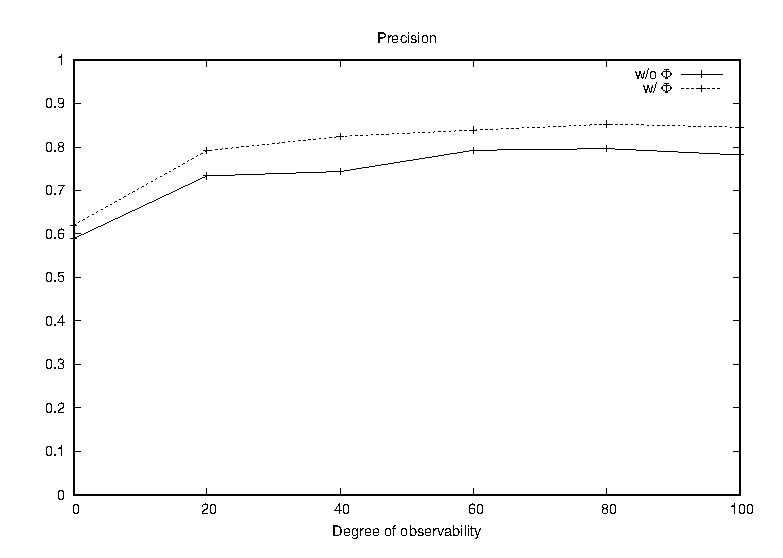
\includegraphics[width=\linewidth]{figures/comparison_precision.eps}
	\caption{Comparison of the precision of the learned models for increasing degrees of observability.}
	\label{fig:comparison_precision}
\end{figure}

\begin{figure}[hbt!]
	\centering
	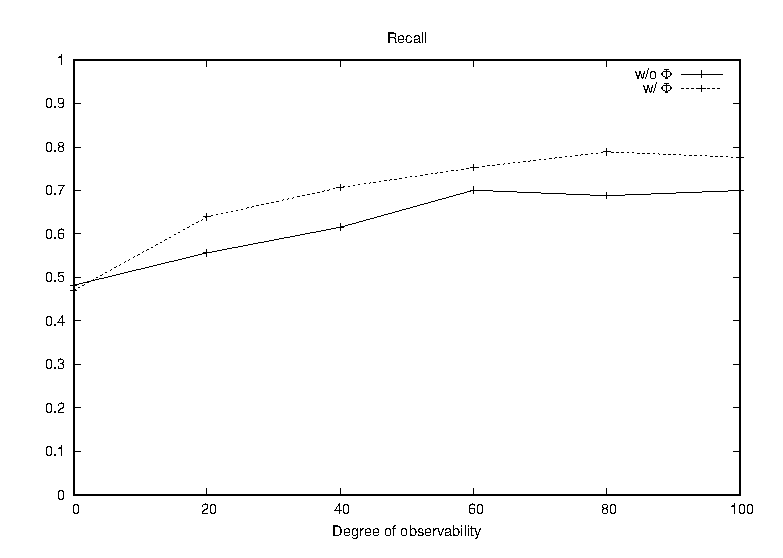
\includegraphics[width=\linewidth]{figures/comparison_recall.eps}
	\caption{Comparison of the recall of the learned models for increasing degrees of observability.}
	\label{fig:comparison_recall}
\end{figure}

Figures \ref{fig:comparison_precision} and \ref{fig:comparison_recall} compare the precision and recall of the learned models in the settings with and without domain knowledge. The values plotted in these figures are averages across all the domains seen in the previous experiment. The results show that using domain knowledge significantly improves the learned models no matter how complete the training examples are. Another interesting aspect is that domain knowledge is able to enrich observations in the range of 30\% observability to the level of fully observable trajectories, which means that domain knowledge can make up for a lack of completeness in the training examples.

\section{Related work}
\label{sec:related}
In {\em Inductive Logic Programming} it is common to make the hypothesis be consistent with the {\em background knowledge}, that is some form {\em deductive knowledge} apart from the examples~\cite{muggleton1994inductive}.

{\em State-invariants} have also been previously used to improve the automatic construction of HTN planning model~\cite{lotinac2016constructing}.

Our learning setting is related to the classical planning formulation where no action model is given~\cite{SternJ17}. This planning setting can can be seen as an scenario when the action model is {\em learned} from a single example that contains only two state observations: the initial state and the goals.




\section{Conclusions}
\label{sec:conclusions}
In some contexts it is however reasonable to assume that the action model is not learned from scratch, e.g. because some parts of the action model are known~\cite{ZhuoNK13,sreedharan2018handling,pereira2018heuristic}. Our compilation is also flexible to this particular learning scenario. The known preconditions and effects are encoded setting the corresponding fluents $\{pre\_e\_\xi, eff\_e\_\xi\}_{\forall e\in{\mathcal I}_{\Psi,\xi}}$ to true in the initial state. Further, the corresponding insert actions, $\mathsf{insertPre_{p,\xi}}$ and $\mathsf{insertEff_{p,\xi}}$, become unnecessary and are removed from $A_{\Lambda}$, making the classical planning task $P_{\Lambda}$ easier to be solved. For example, suppose that the preconditions of the {\em blocksworld} action schema {\tt stack} are known, then the initial state is extended with literals, {\small\tt(pre\_holding\_v1\_stack)} and {\small\tt(pre\_clear\_v2\_stack)} and the associated actions $\mathsf{insertPre_{holding_v1,stack}}$ and $\mathsf{insertPre_{clear_v2,stack}}$ can be safely removed from the $A_{\Lambda}$ action set without altering the {\em soundness} and {\em completeness} of the $P_{\Lambda}$ compilation.

%% The file named.bst is a bibliography style file for BibTeX 0.99c
\bibliographystyle{named}
\bibliography{planlearnbibliography}

\end{document}
